\chapter{Caso de estudio}
\label{chap:case-study}

\section{Introducción}
\label{sec:5:introduction}

En este capítulo vamos a describir los casos de uso principales de ChatStats. Estas descripciones cubrirán todas las funciones principales, así como una descripción detallada de los pasos a seguir y cómo usar la aplicación.

A lo largo de los casos de uso, iremos viendo la aplicación en distintos dispositivos y tamaños, pudiendo comprobar cómo la aplicación se adapta a la pantalla de una forma \textit{responsive}.

\section{Instalar aplicación en cliente}

En esta sección se explicará el proceso de instalación de ChatStats en un dispositivo con navegador con soporte para \acrfull{pwa}.

En primer lugar, el usuario accede a la web donde se aloja la aplicación. El navegador sugiere la instalación de la aplicación. El usuario pulsa sobre la sugerencia e instala la aplicación, que estará accesible desde el escritorio del dispositivo. La aplicación puede usarse sin acceso a Internet.


\begin{figure}[H]
	\centering
	\subfloat[\centering Acceso a ChatStats]{{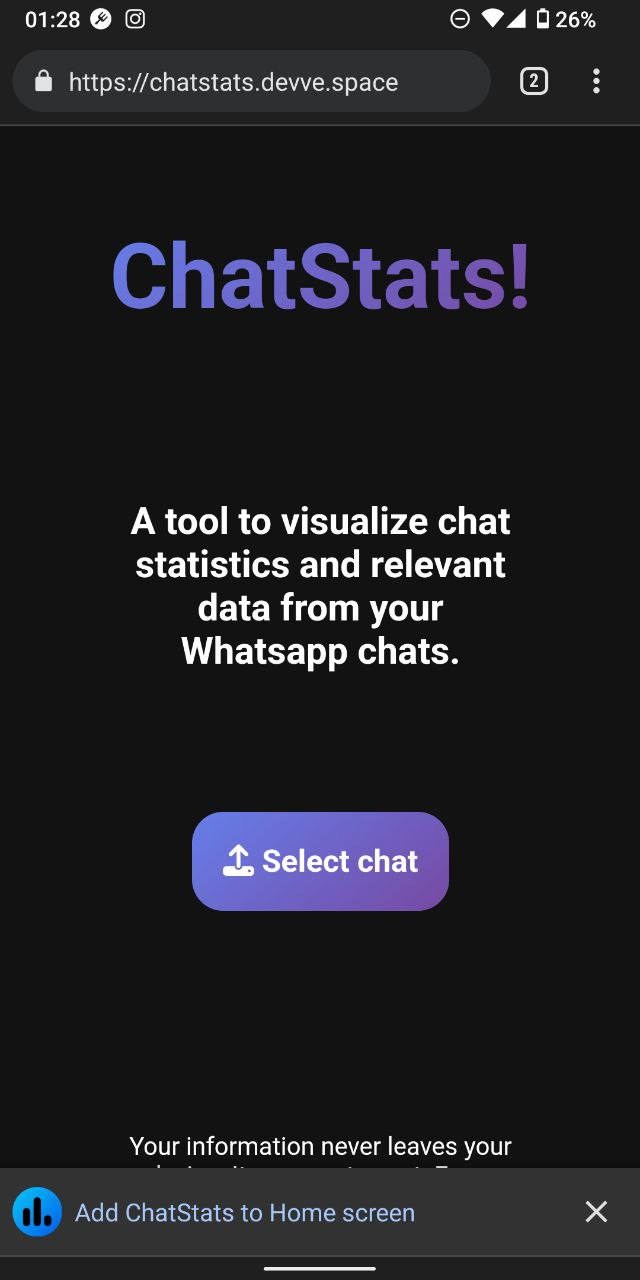
\includegraphics[width=3cm]{img/study_case/installation_1.jpg} }}
	\qquad
	\subfloat[\centering Instalación]{{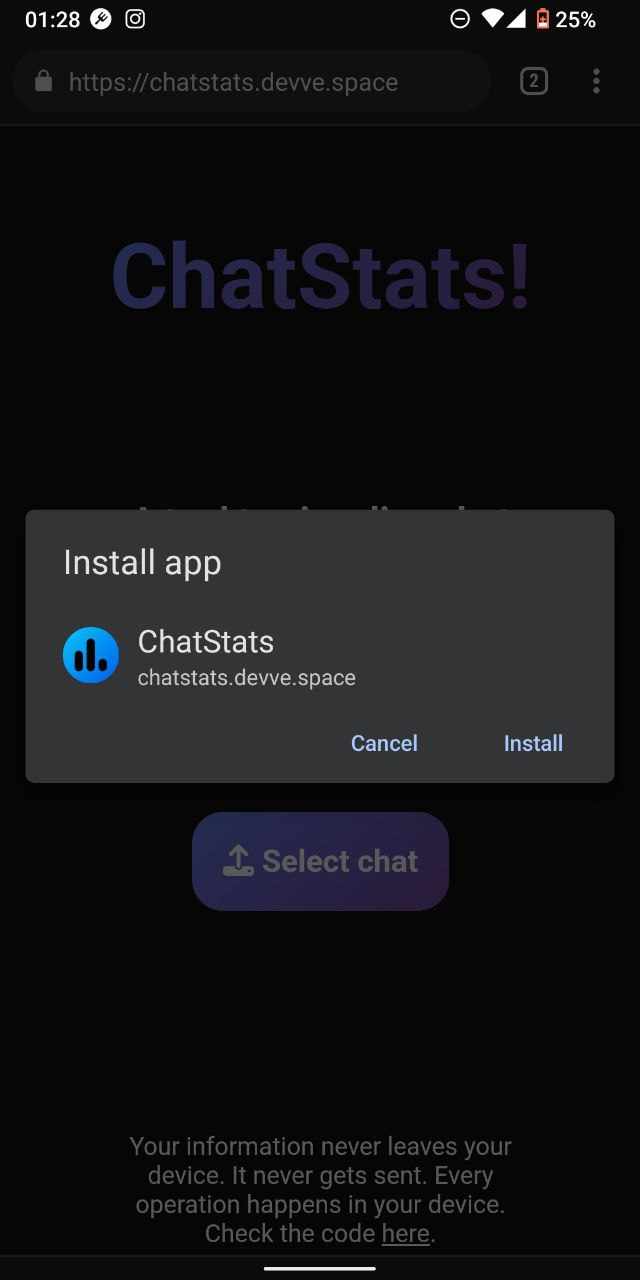
\includegraphics[width=3cm]{img/study_case/installation_2.jpg} }}
	\qquad
	\subfloat[\centering Colocación en escritorio]{{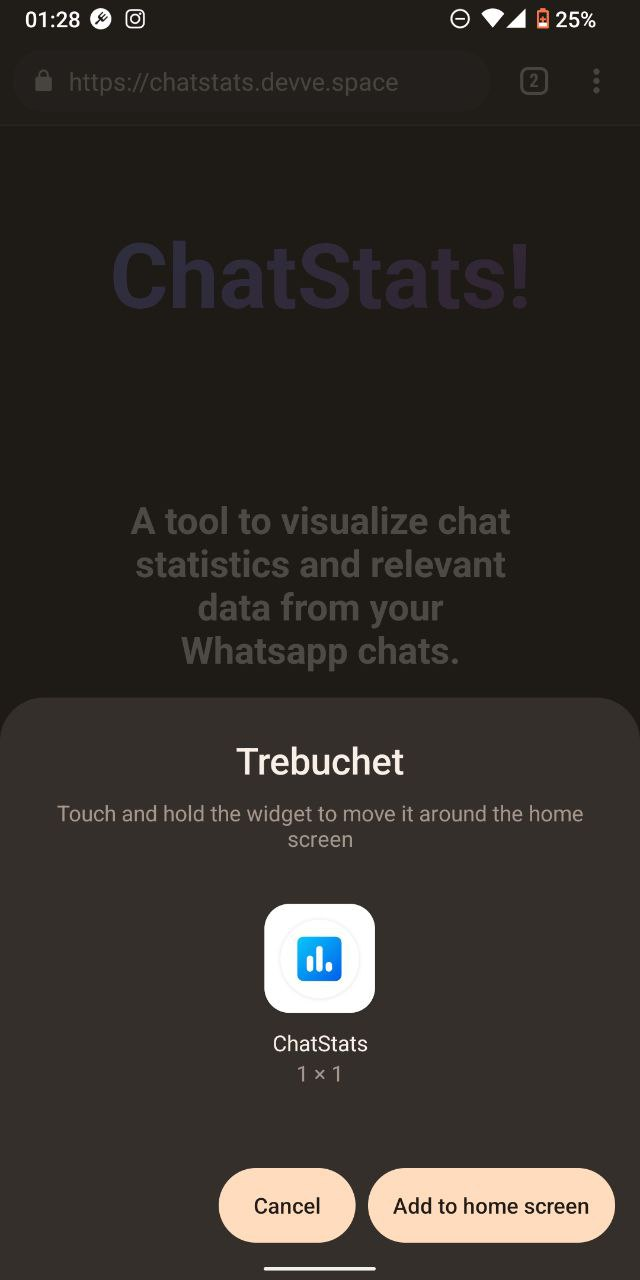
\includegraphics[width=3cm]{img/study_case/installation_3.jpg} }}
	\caption{Instalación de la aplicación \acrshort{pwa}}
	\label{fig:chap5:pwa_installation}
\end{figure}


\section{Importar datos en el sistema}

Durante este caso de uso, el usuario puede seleccionar un archivo para importar a ChatStats. El archivo puede ser de texto plano, \textit{zip} o \acrshort{json}. En caso de ser otro tipo de archivo, ChatStats alerta al usuario y elimina la selección.

\begin{figure}[H]
	\centering
	\subfloat[\centering Selección de fichero]{{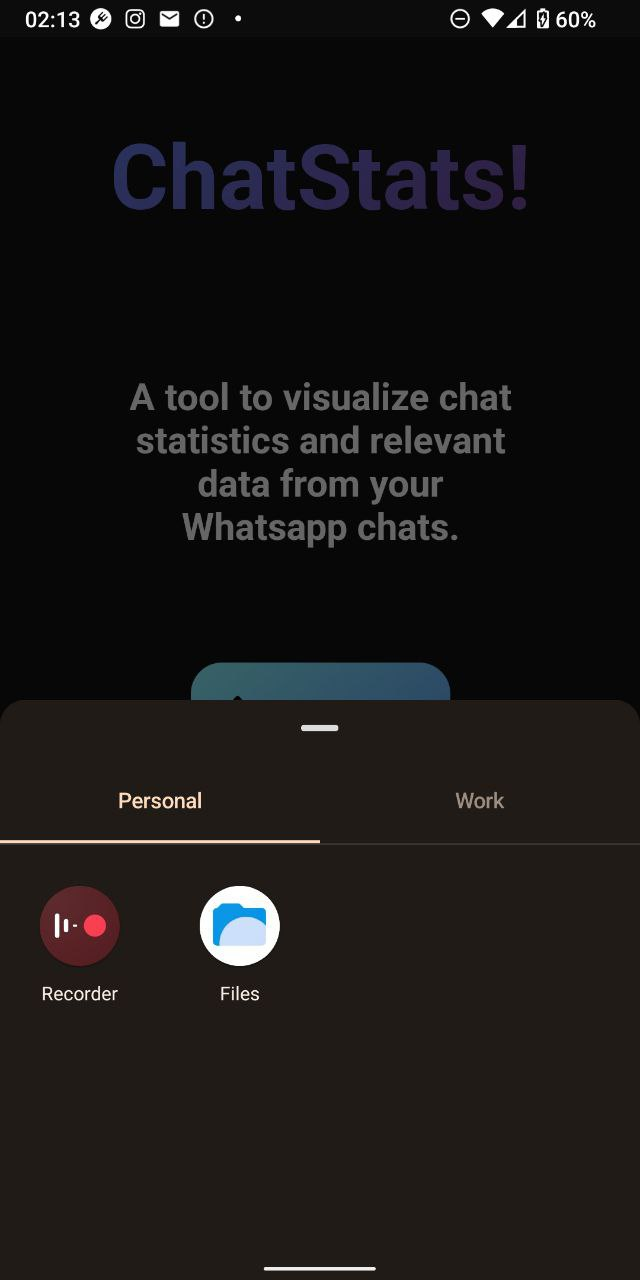
\includegraphics[width=3cm]{img/study_case/import_1.jpg} }}
	\qquad
	\subfloat[\centering Fichero válido seleccionado]{{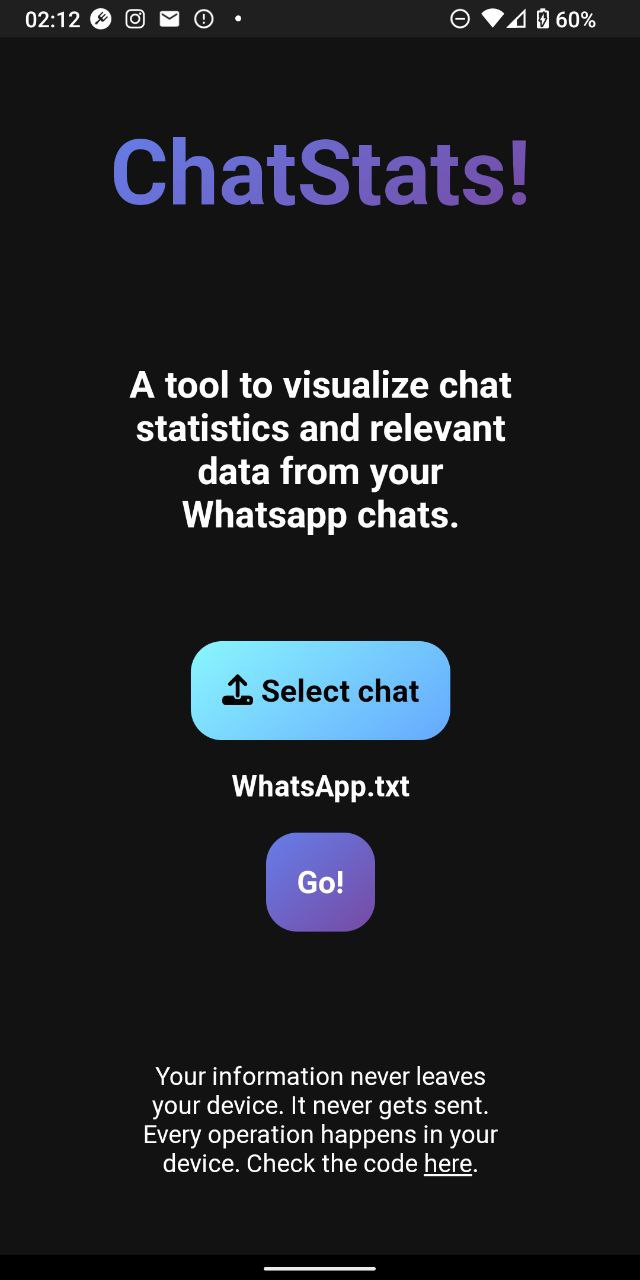
\includegraphics[width=3cm]{img/study_case/import_2.jpg} }}
	\qquad
	\subfloat[\centering Fichero no válido seleccionado]{{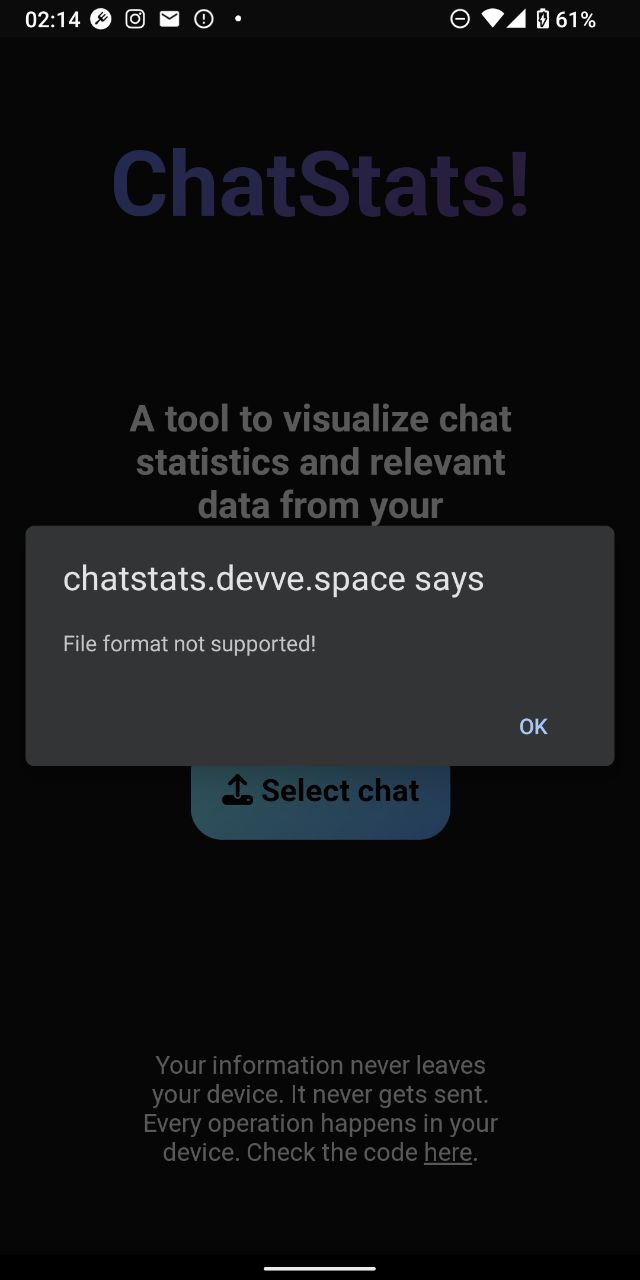
\includegraphics[width=3cm]{img/study_case/import_3.jpg} }}
	\caption{Importar datos en el sistema}
	\label{fig:chap5:import}
\end{figure}


\section{Visualización de chat grupal e individual}

\subsection{Cálculo de las estadísticas}

Durante esta pantalla, el cliente está ejecutando todos los flujos descritos en el \autoref{chap:architecture}. Se muestra una animación de carga para hacer saber al usuario que el cliente está realizando operaciones.

\begin{figure}[H]
	\centering
	\subfloat[\centering Inicio del cálculo]{{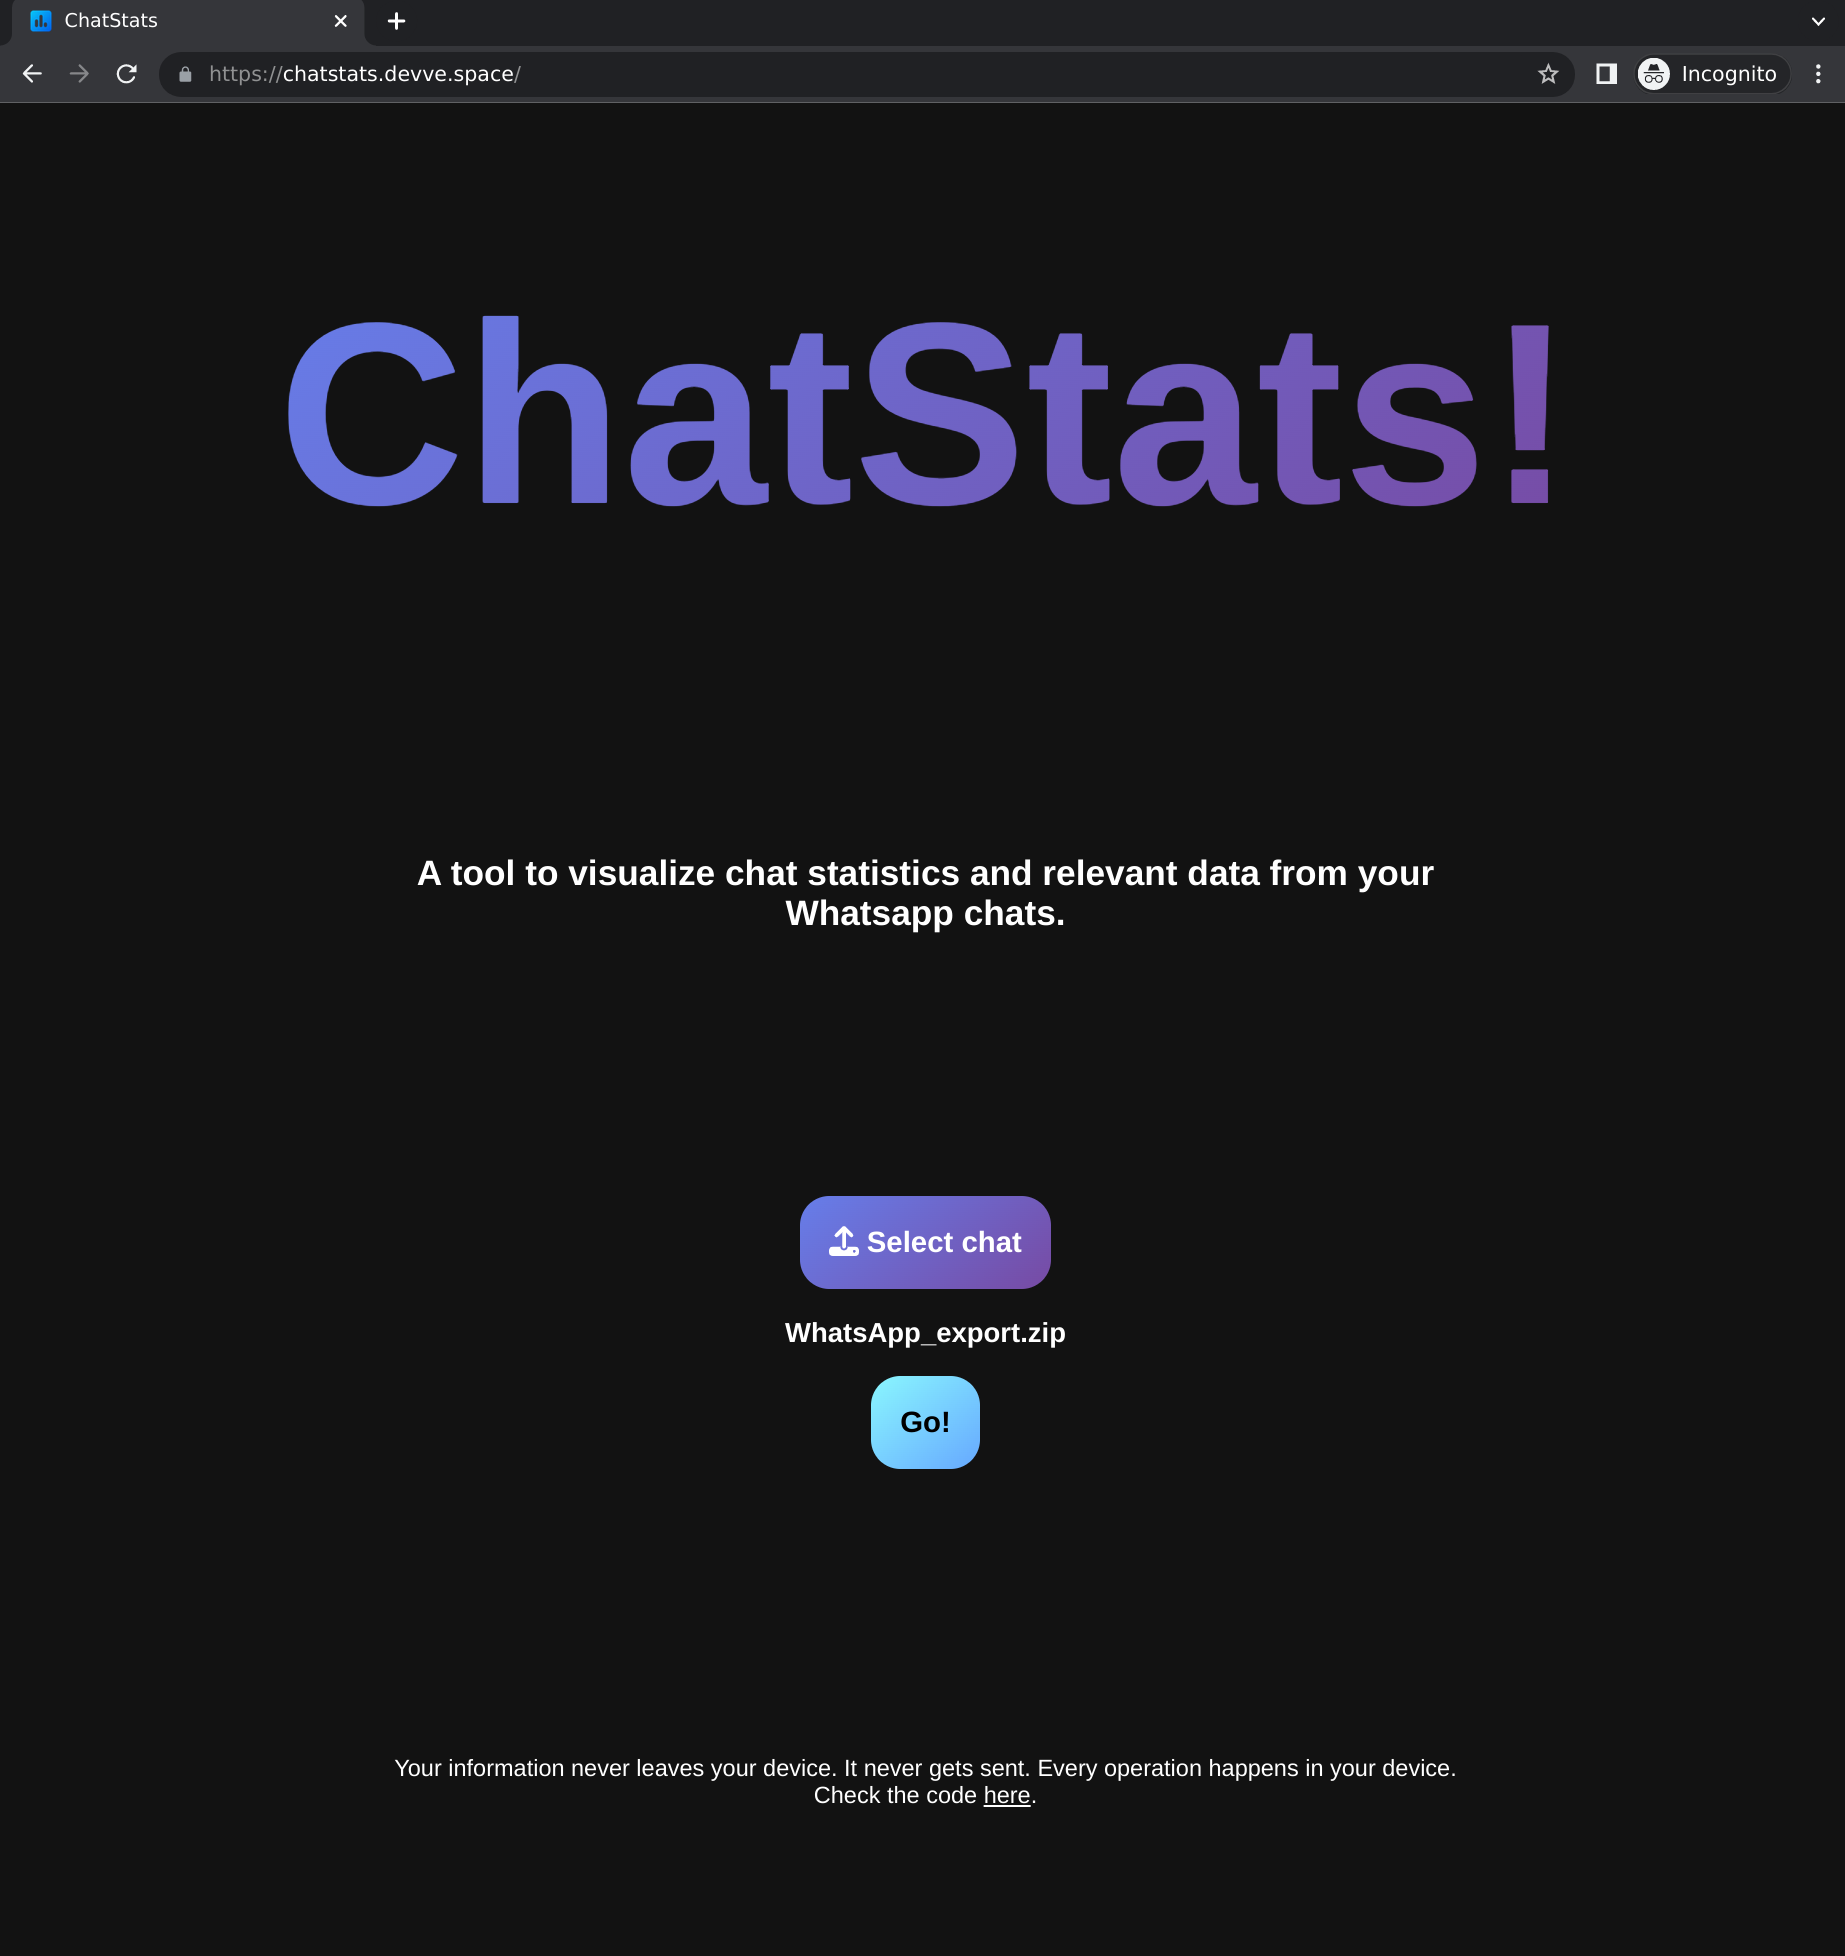
\includegraphics[width=7.1cm]{img/study_case/metrics_calc_1.png} }}
	\qquad
	\subfloat[\centering Carga durante el cálculo de métricas]{{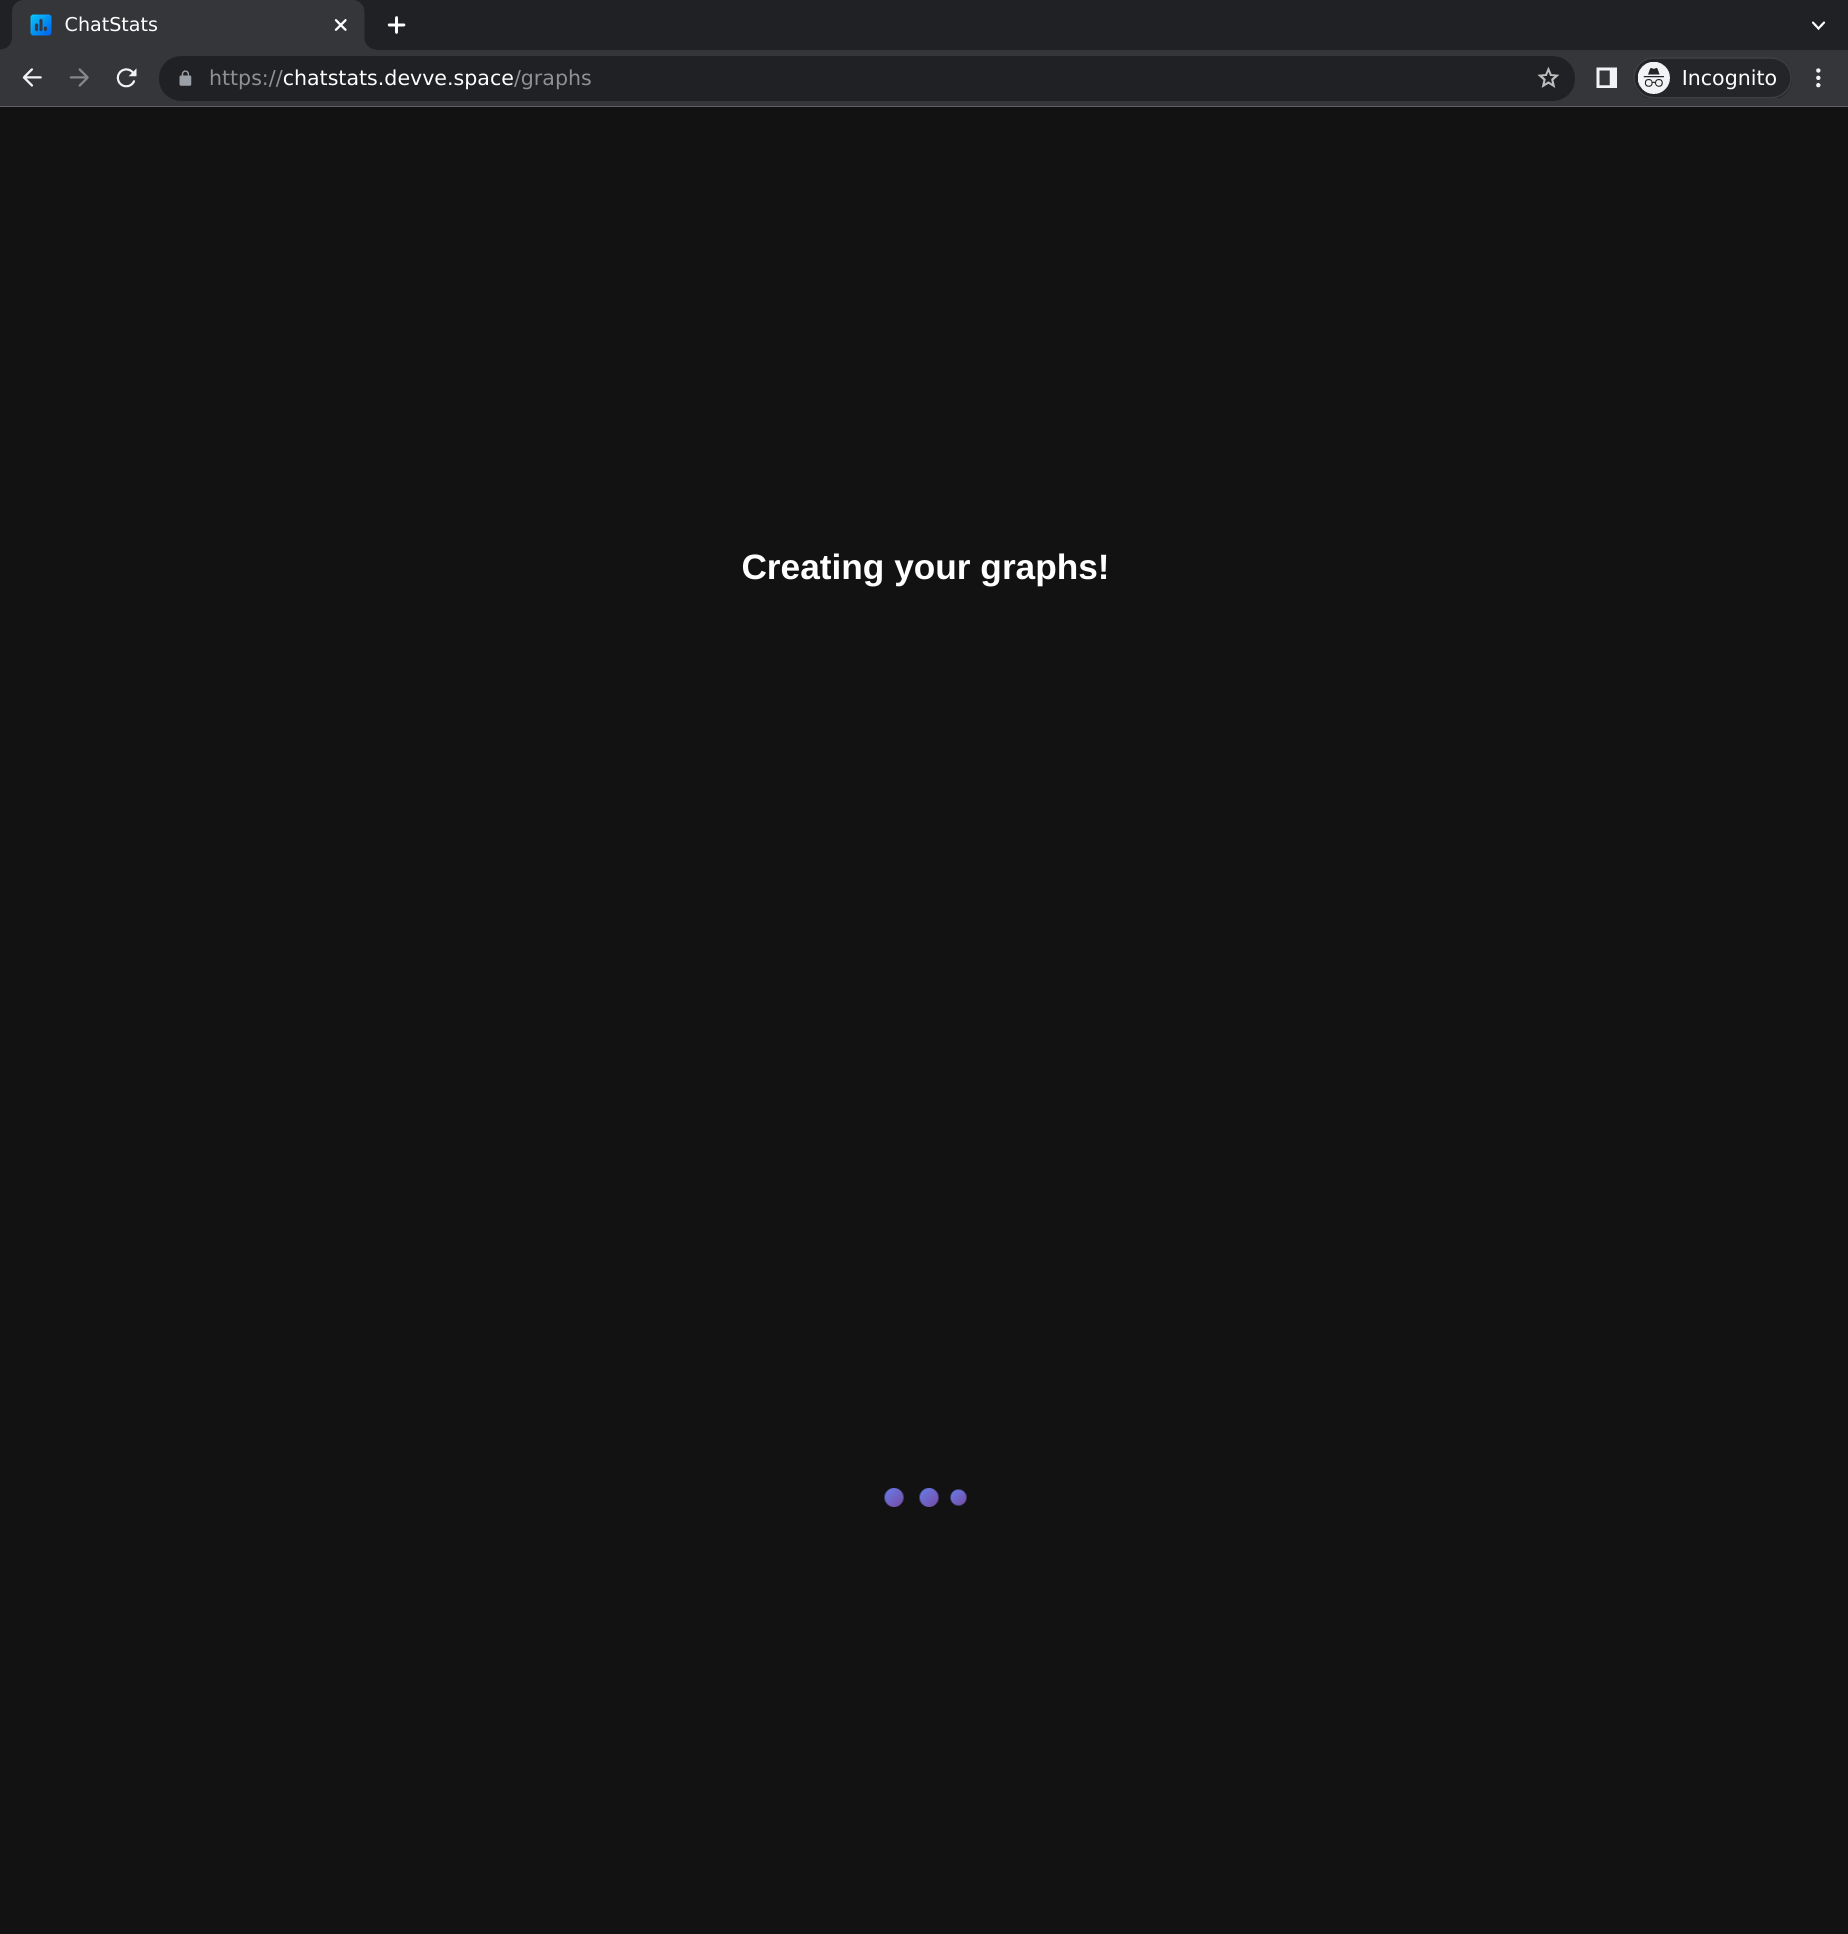
\includegraphics[width=7.1cm]{img/study_case/metrics_calc_2.png} }}
	\caption{Cálculo de métricas}
	\label{fig:chap5:calc}
\end{figure}


\subsection{Visualización de chat grupal e individual}

En esta página se muestran numerosos gráficos descritos durante la arquitectura, por los que el usuario puede desplazarse mediante la navegación vertical.

En el primer grupo de gráficos de la \autoref{fig:chap5:viz_grupal} (a) observamos el recuento de mensajes, palabras y caracteres para cada contacto. En este caso, podemos apreciar como los usuarios ``Alejandro'' y ``James'', en azul y morado respectivamente, constituyen casi un tercio de la conversación.

En el grupo de gráficos (b), en la \autoref{fig:chap5:viz_grupal} podemos observar la media de palabras por mensaje, así como la media de caracteres. De ellos podemos concluir, en este ejemplo, que todos los contactos escriben en media mensajes del mismo tamaño. En este grupo se incluye también un gráfico que indica el número de veces que cada contacto ha iniciado la conversación; así como el tiempo medio de respuesta de cada uno. Estos datos pueden ser muy útiles para medir el interés de los contactos por el chat en cuestión, así como qué contacto tiene mayor iniciativa al diálogo. Para nuestro caso de ejemplo, se observa que ``Alejandro'' suele comenzar la conversación, así como que Adriana es muy rápida respondiendo.

Continuando con el grupo de gráficos (c), podemos observar el número de archivos multimedia de cada tipo que ha enviado cada contacto. Aquí vemos que ``Adriana'' manda muchas pegatinas o \textit{stickers}, mientras que ``Jaime'' acostumbra a mandar más audios.

En el grupo de gráficos (d), podemos observar las distribución de los mensajes en los meses, en los días de la semana y en las horas del día. Anotamos que diciembre de 2022 fue el mes más activo del grupo y que los lunes suelen tener mayor actividad (que va decayendo a lo largo de la semana). Cabe comentar que en todos los gráficos anteriores se pueden descartar contactos en la representación. Es por eso que, quedándonos con ``James'' y ``Jaime'', podemos observar que ``James'' suele comenzar a enviar mensajes una hora antes que ``Jaime''.

Finalmente, en el grupo de gráficos (e) podemos observar las palabras clave más frecuentes del chat, así como los emoticonos. Estos nos permiten conocer rápidamente los temas principales de conversación, que son, en este caso: \textit{Google}, \textit{GDSC (Google Developers Student Club)} y \textit{evento}, entre otros. Asimismo, los emoticonos nos permiten conocer las principales reacciones no verbales que tienen lugar en la conversación.

\vspace{8mm}

Para el caso de chats individuales, se elimina la necesidad de la utilización de un gráfico circular y se muestran los números calculados directamente. Los gráficos de barras para las distribuciones en el tiempo no varían. Se muestran algunas diferencias en la \autoref{fig:chap5:viz_individual}.

\begin{figure}[h]
	\centering
	\subfloat[\centering Número de mensajes, número de palabras y número de caracteres]{{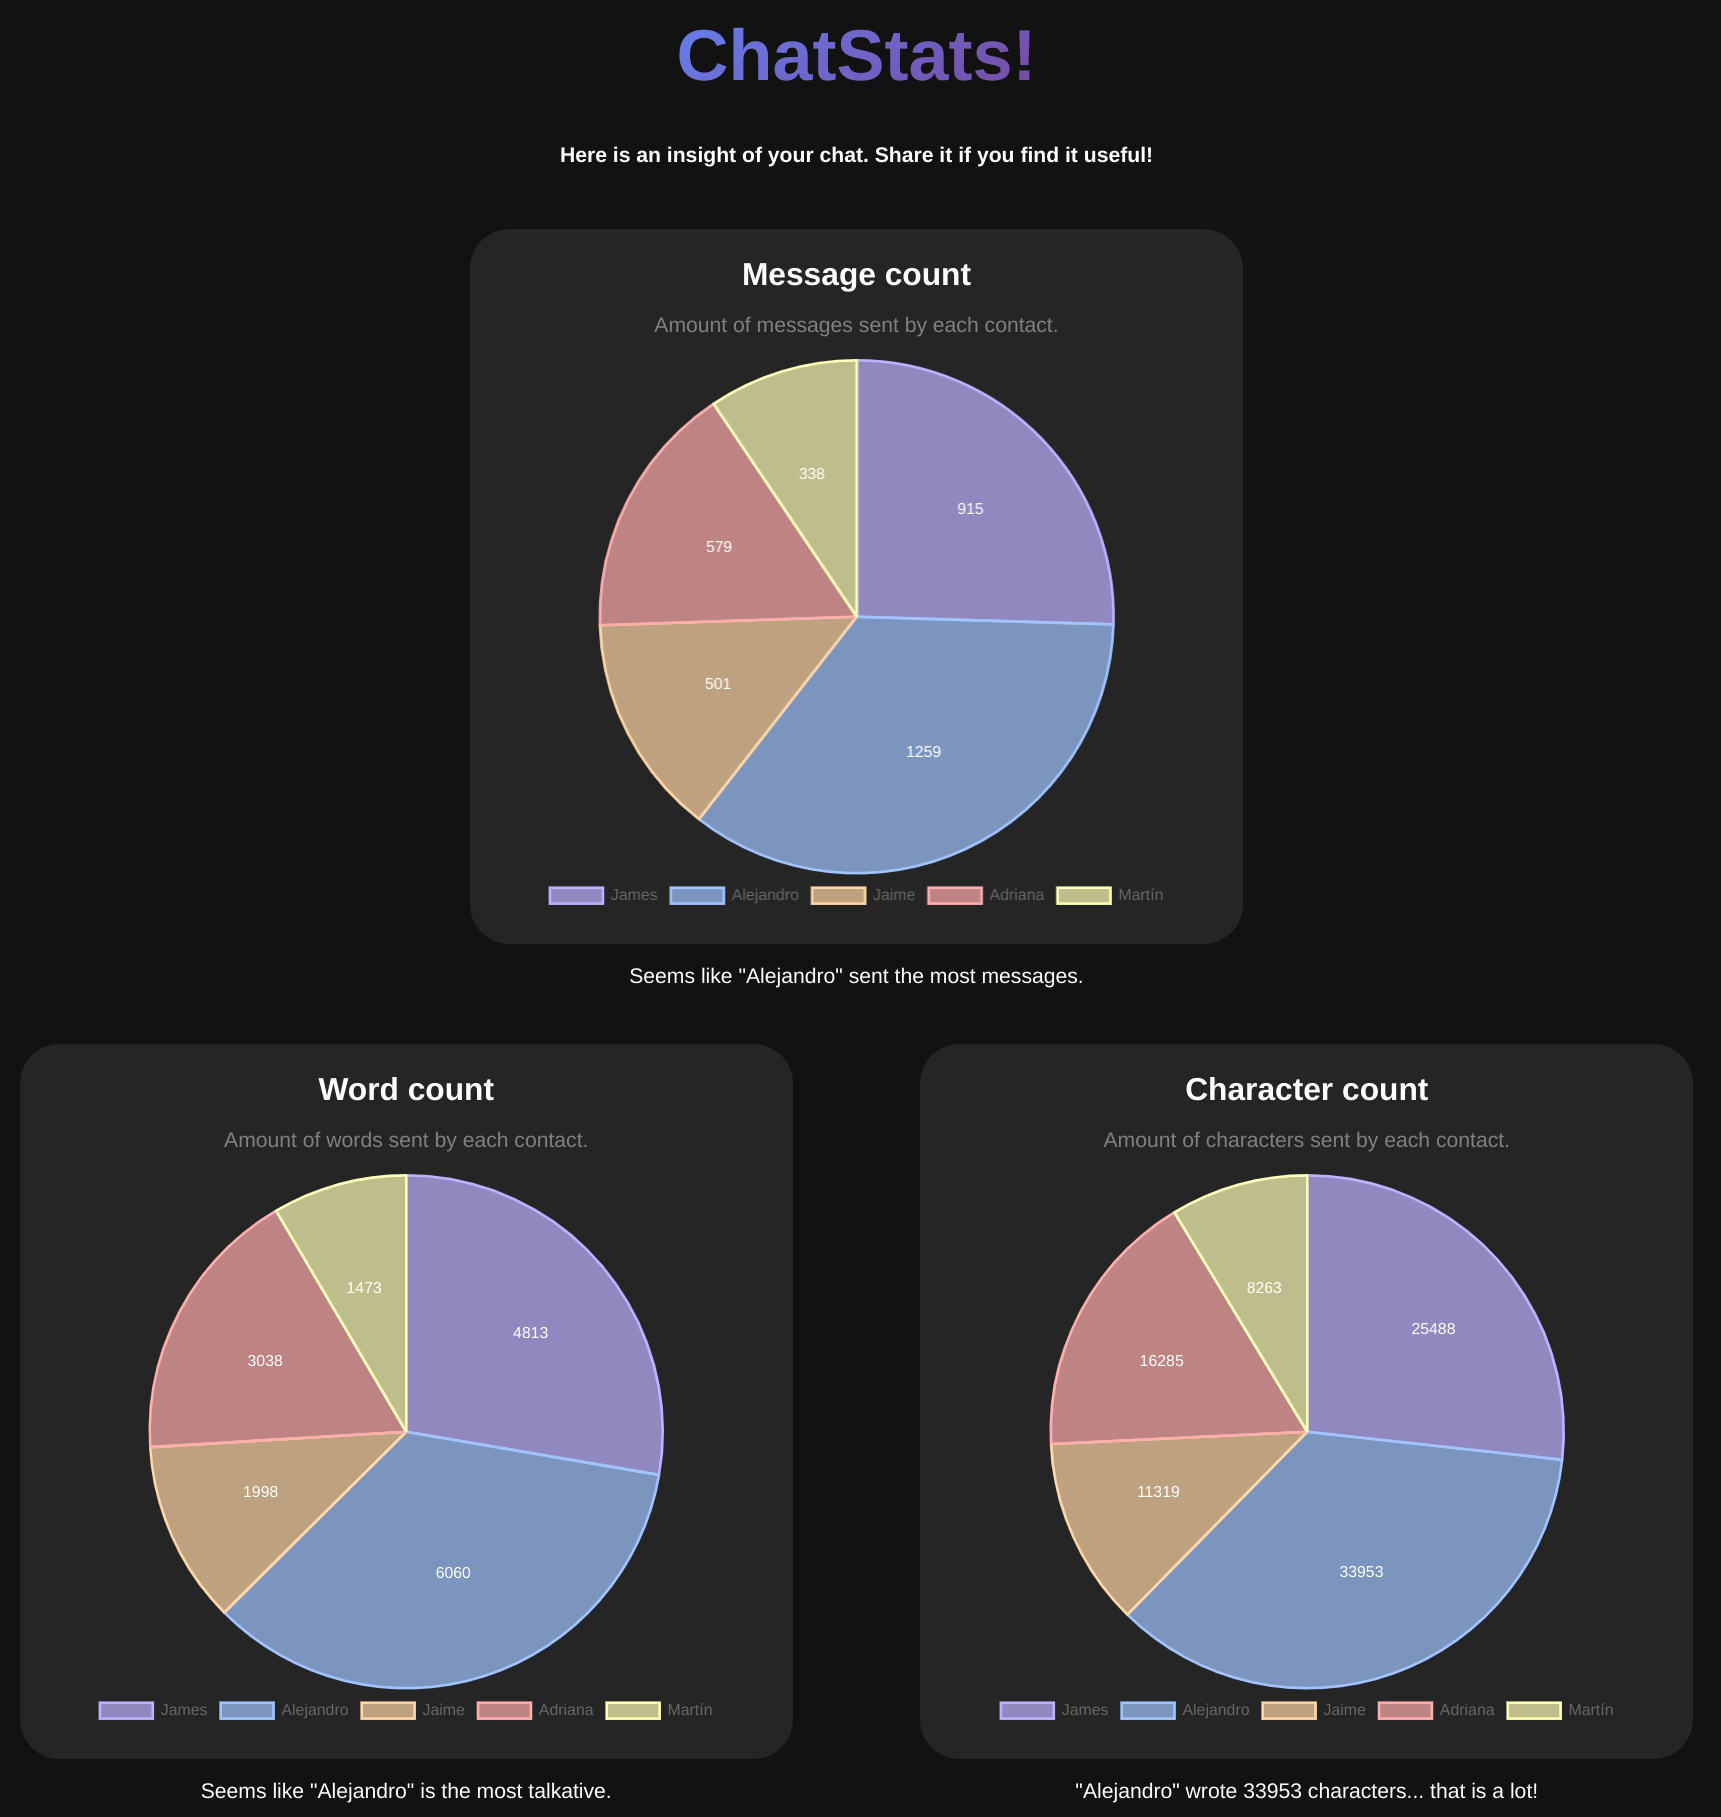
\includegraphics[width=7cm]{img/study_case/screen_1.png} }}
	\qquad
	\subfloat[\centering Media de palabras, media de caracteres, conversaciones iniciadas y tiempo medio de respuesta]{{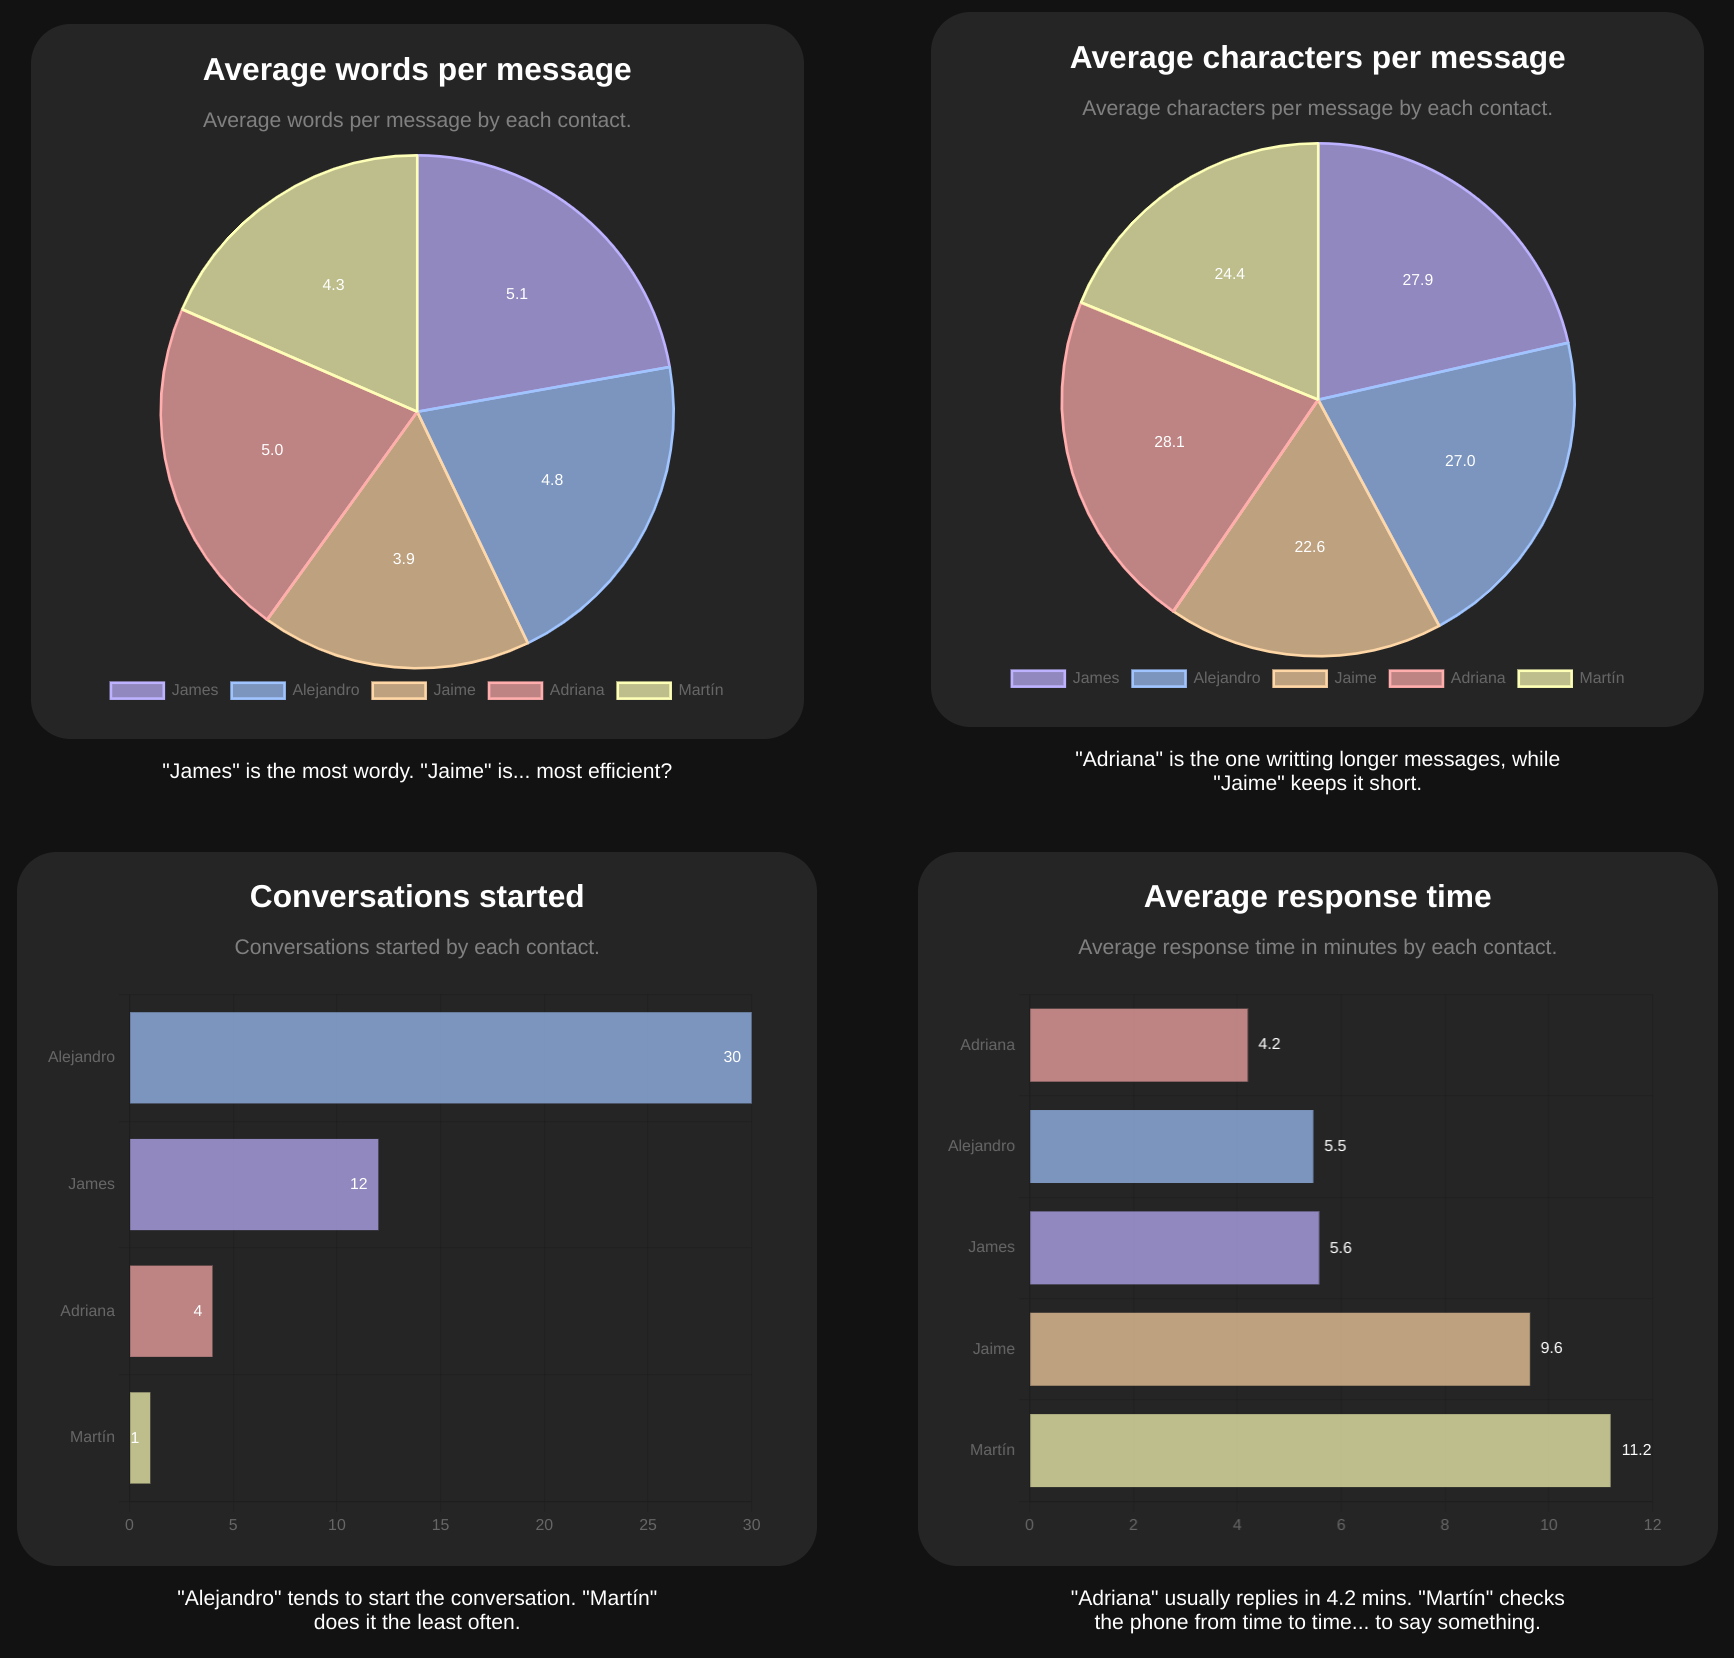
\includegraphics[width=7cm]{img/study_case/screen_2.png} }}
	\centering
	
	
	\subfloat[\centering Número de fotos, vídeos, audios y pegatinas]{{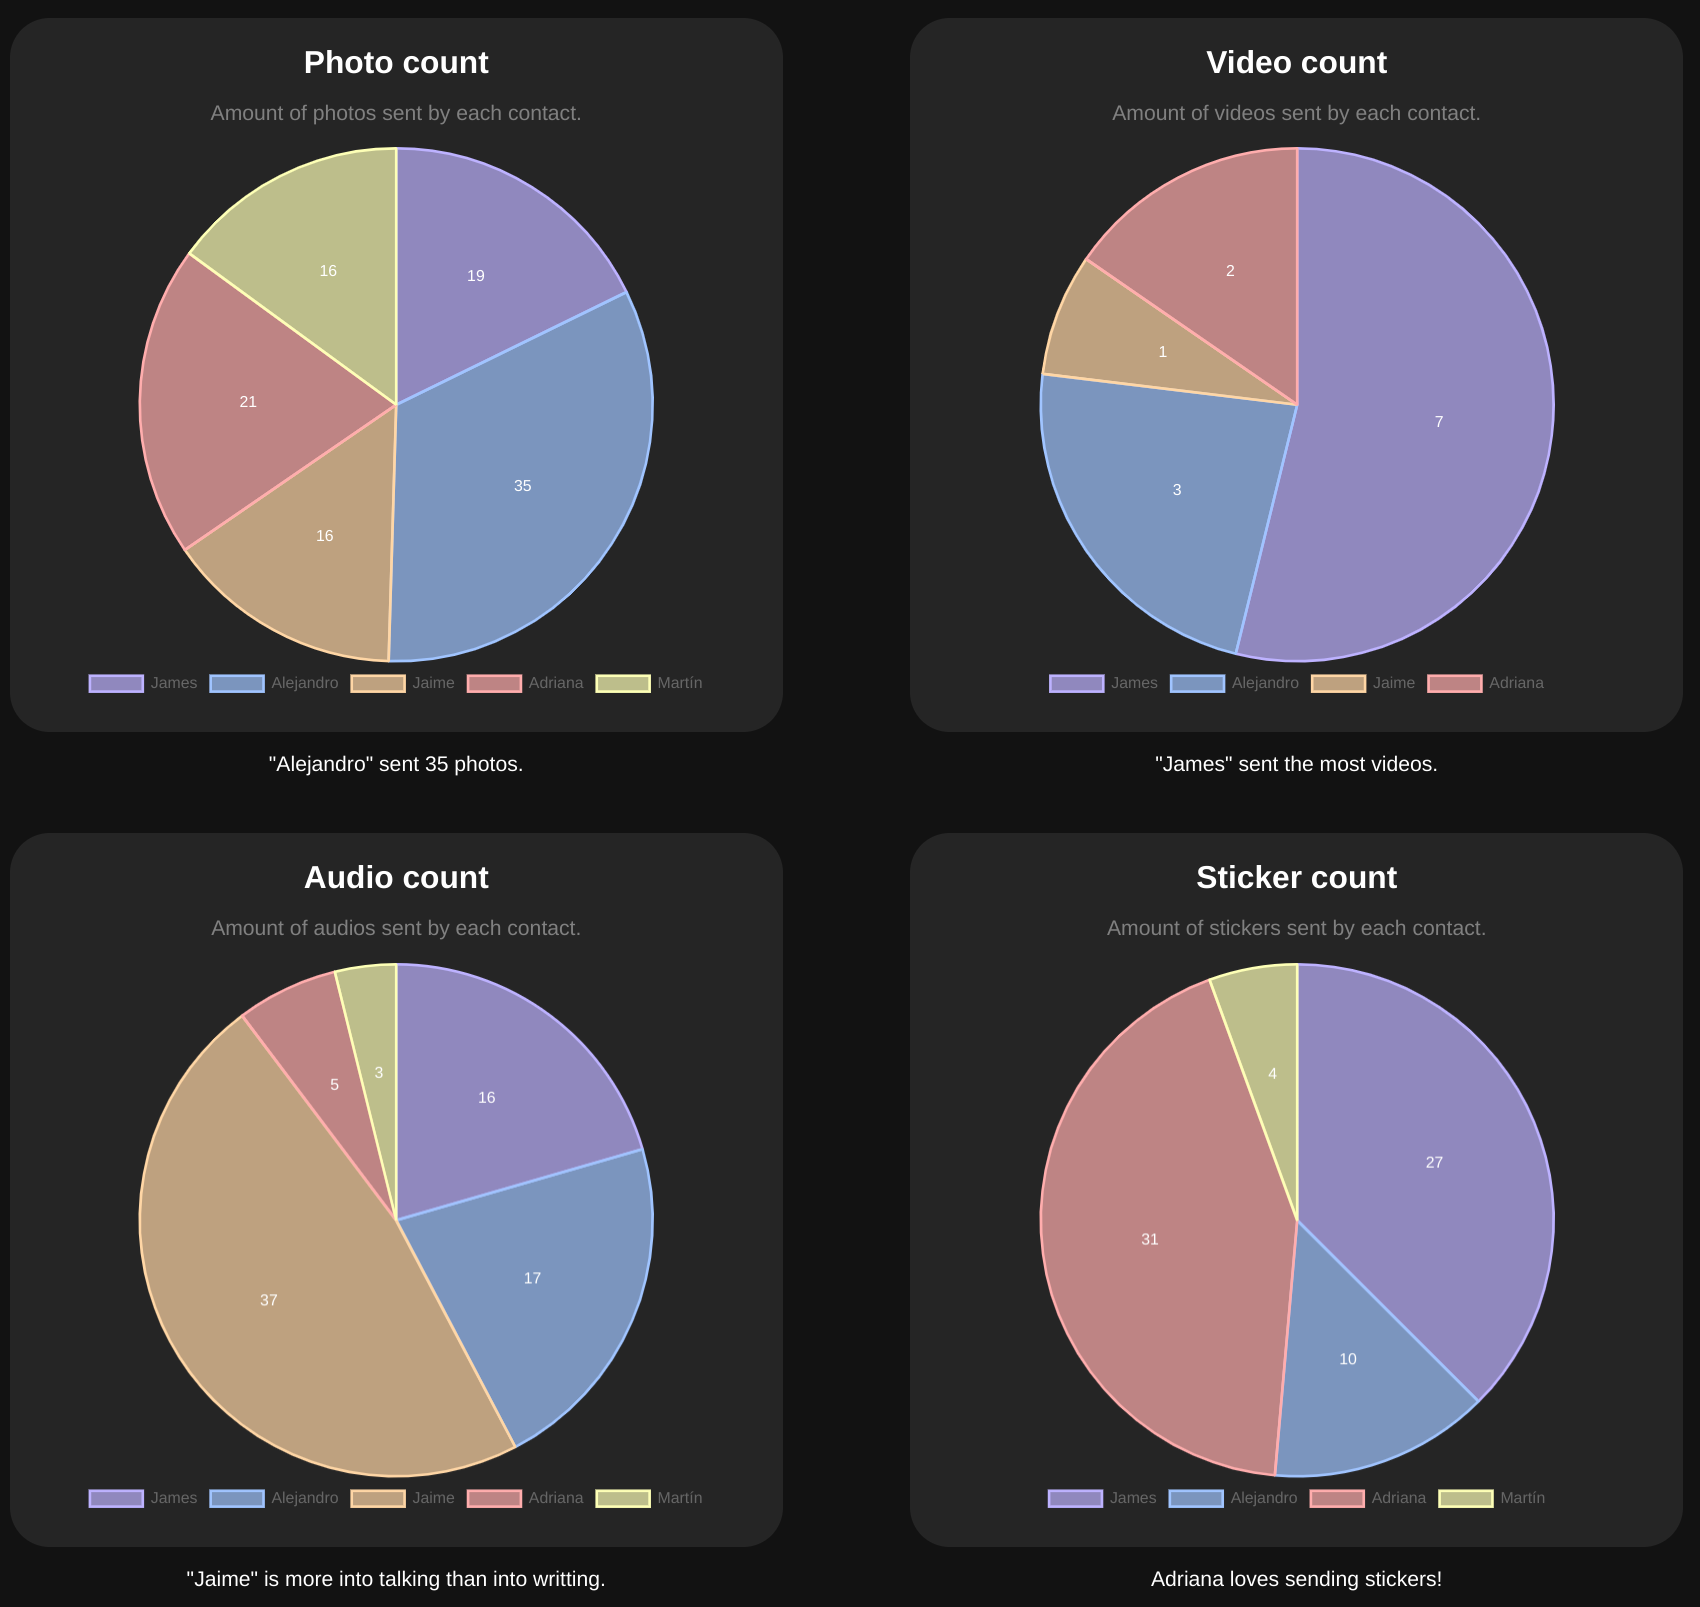
\includegraphics[width=7cm]{img/study_case/screen_3.png} }}
	\qquad
	\subfloat[\centering Distribución de mensajes en meses, días de la semana y  horas del día]{{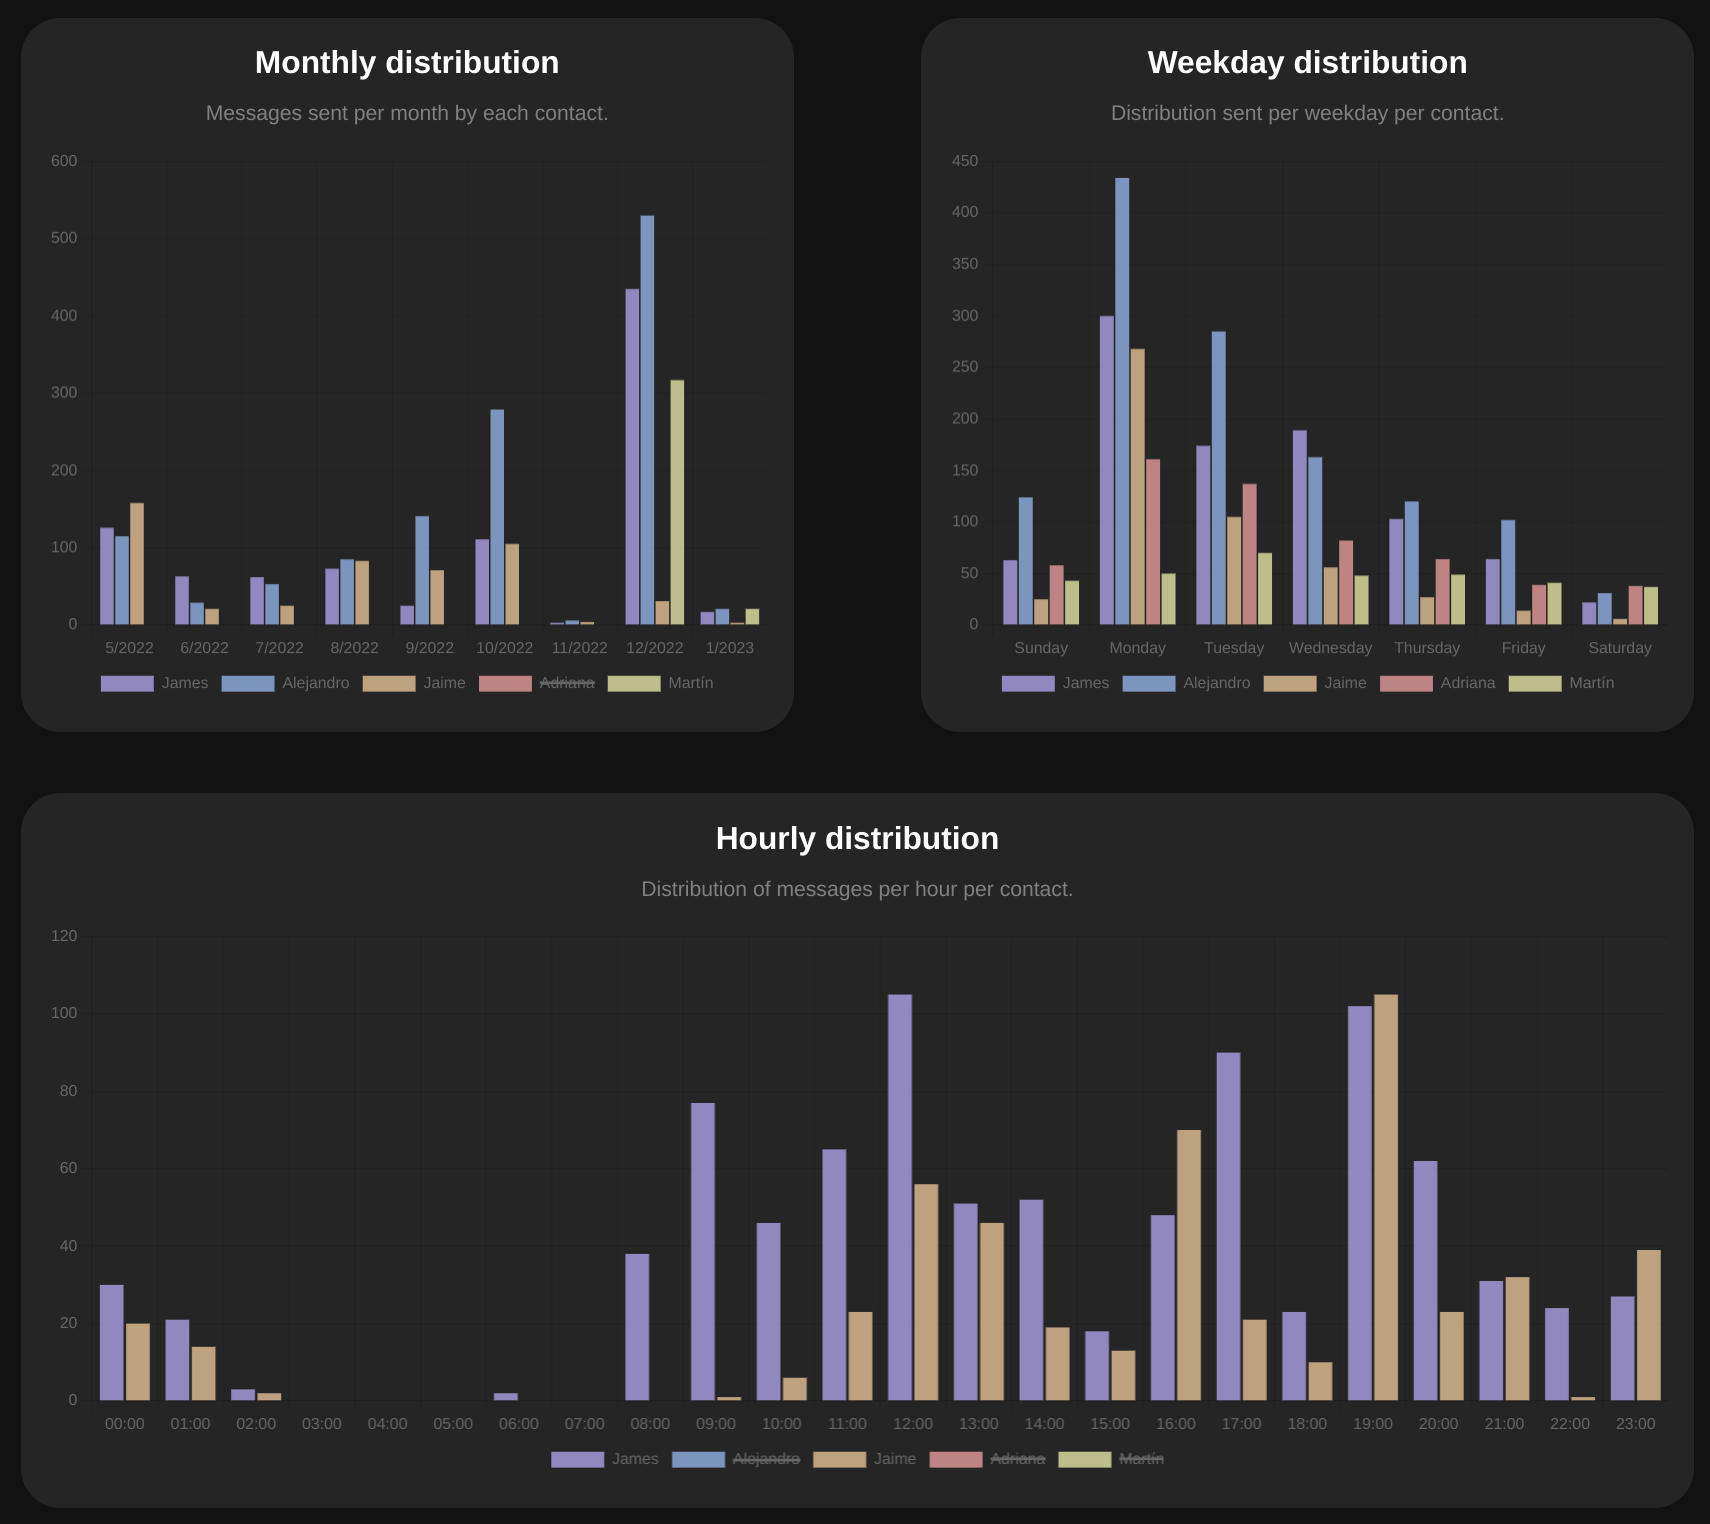
\includegraphics[width=7cm]{img/study_case/screen_4.png} }}
	
	
	\qquad
	\subfloat[\centering Nubes de palabras y emoticonos]{{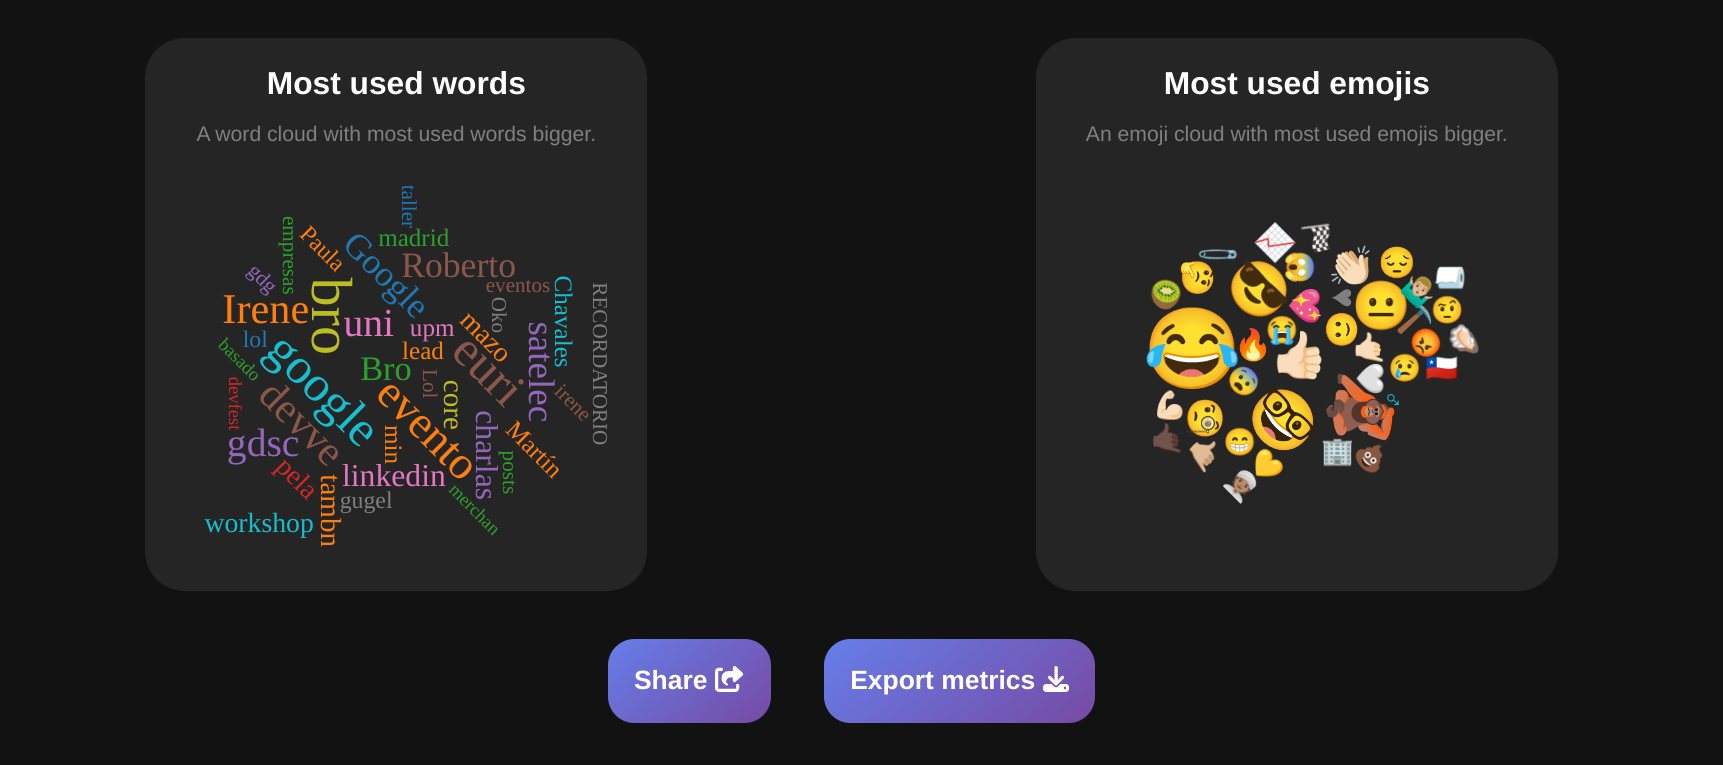
\includegraphics[width=9cm]{img/study_case/screen_5.png} }}
	
	
	\caption{Visualización de chat grupal}
	\label{fig:chap5:viz_grupal}
\end{figure}


\begin{figure}[h]
	\centering
	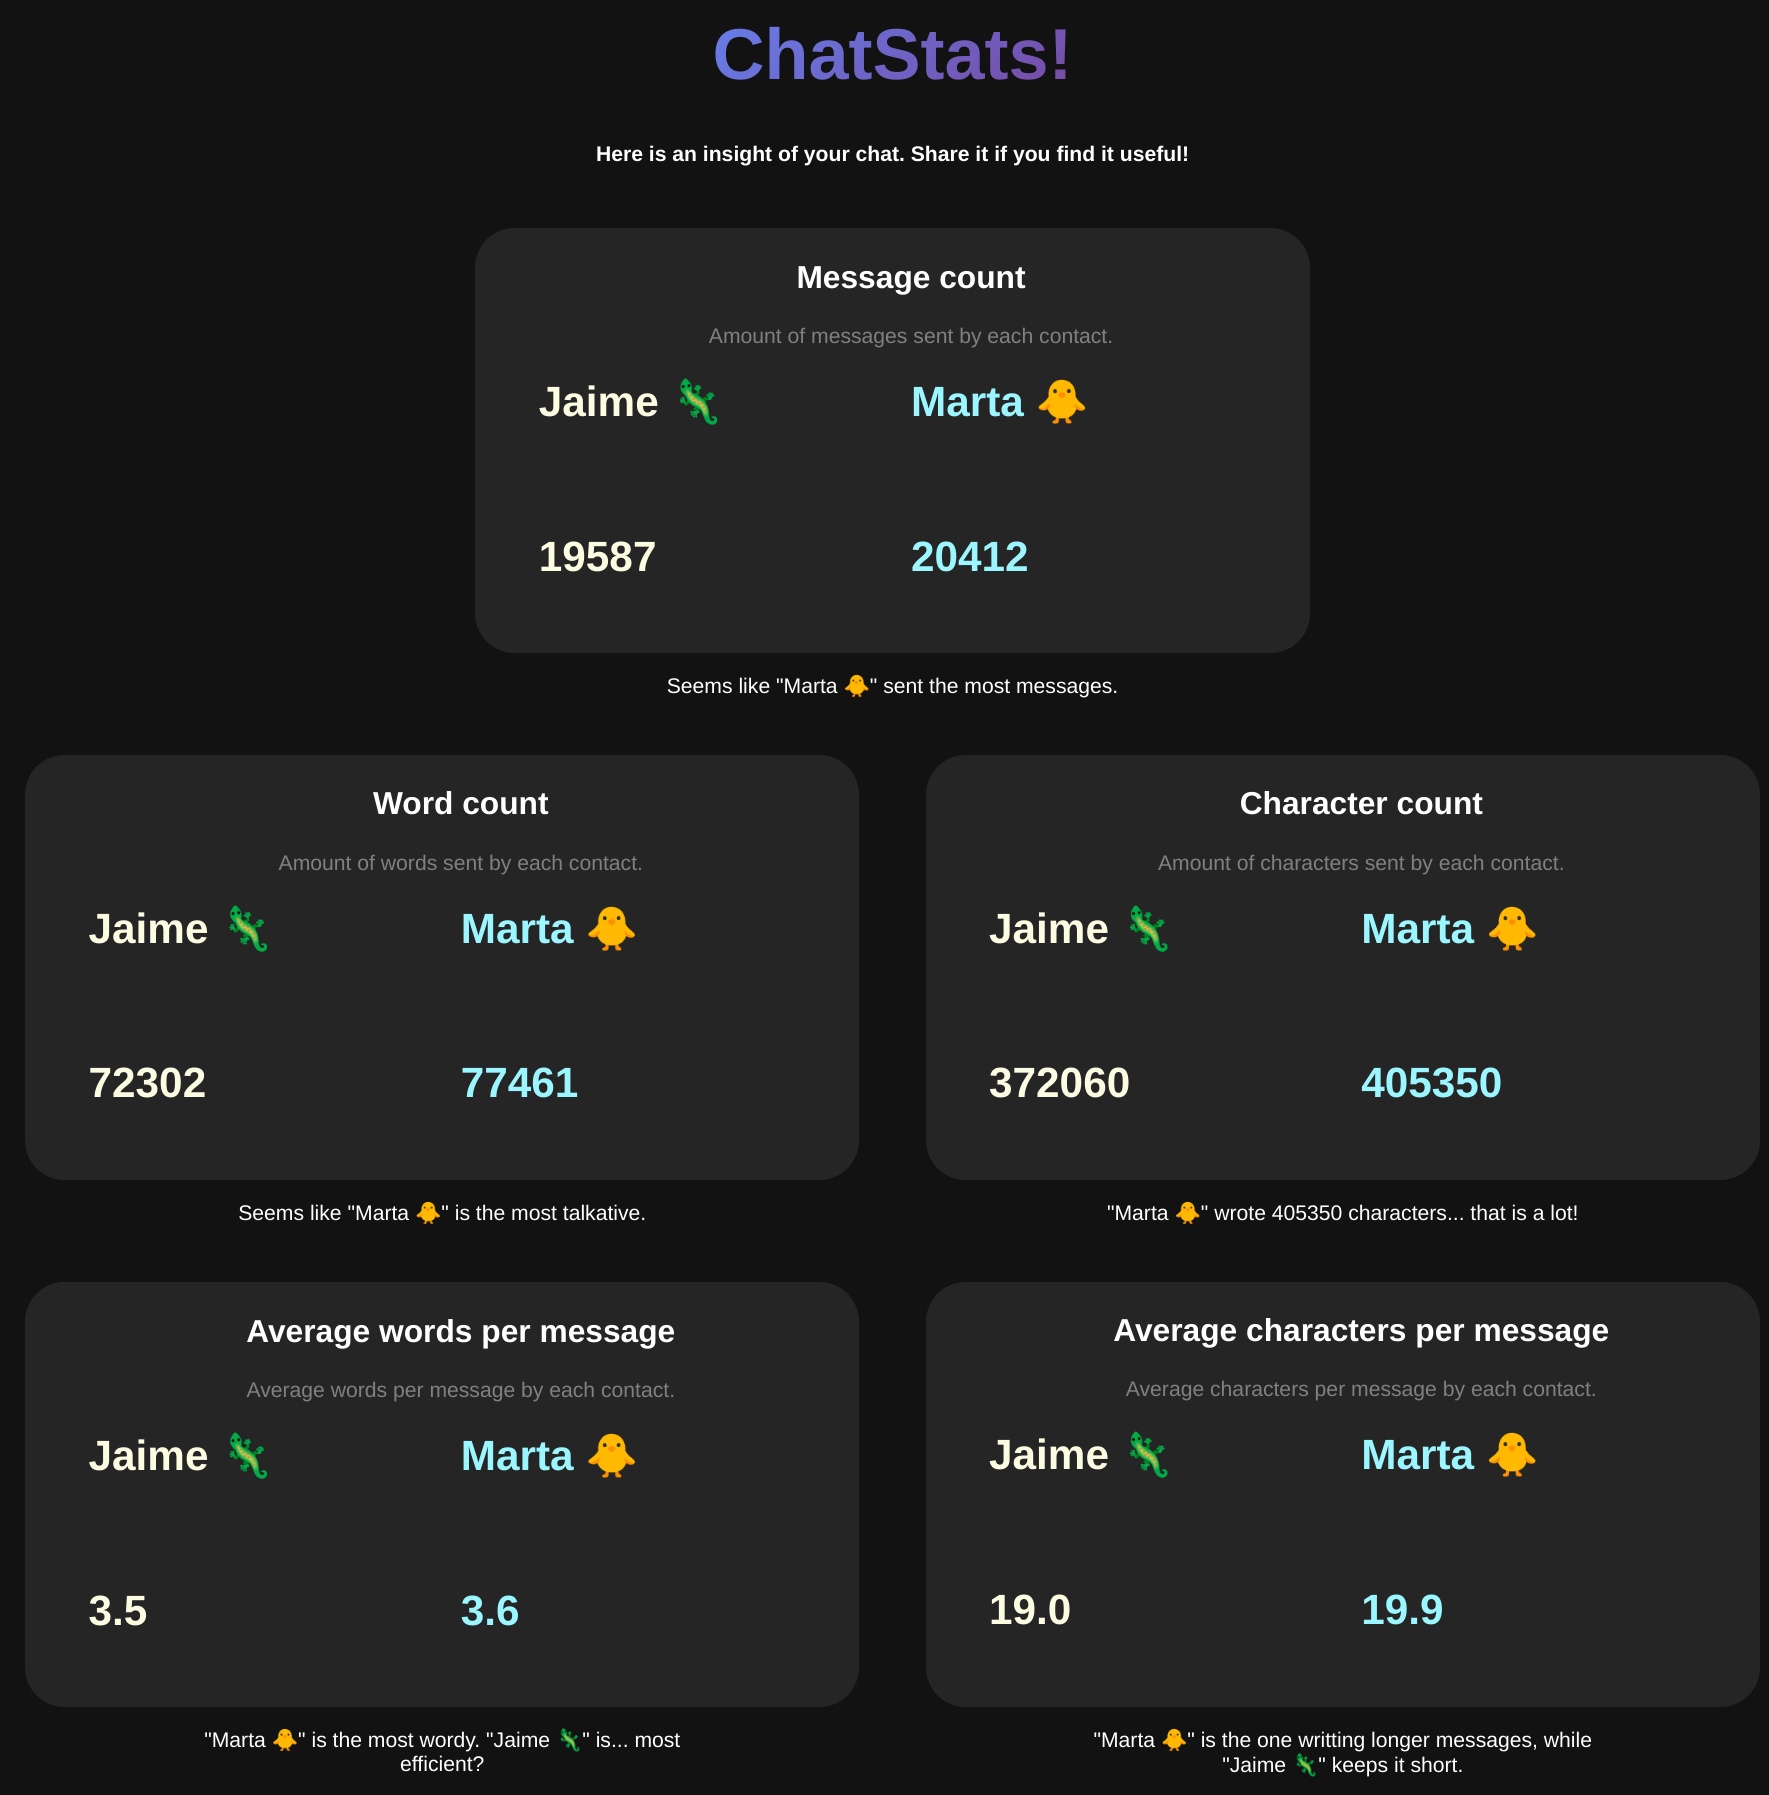
\includegraphics[width=0.6\textwidth]{img/study_case/screen_6.png}
	\caption{Ejemplo de variación para chat individual}
	\label{fig:chap5:viz_individual}
\end{figure}

\section{Exportar analíticas}

Como puede observarse en la \autoref{fig:chap5:export}, se ofrece la opción, al final de la visualización, de exportar una imagen para compartir; así como de exportar las métricas calculadas para su posterior análisis personal.

\begin{figure}[h]
	\centering
	\subfloat[\centering Compartir imagen]{{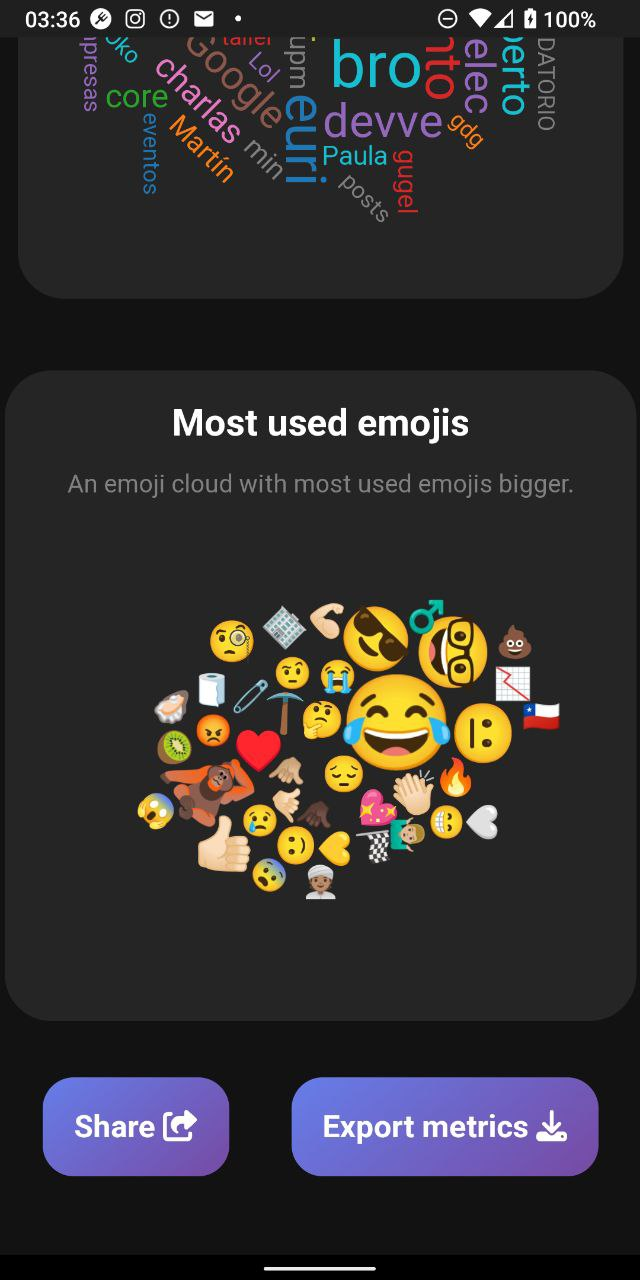
\includegraphics[width=5cm]{img/study_case/export_1.jpg} }}
	\qquad
	\subfloat[\centering Descarga del archivo exportado]{{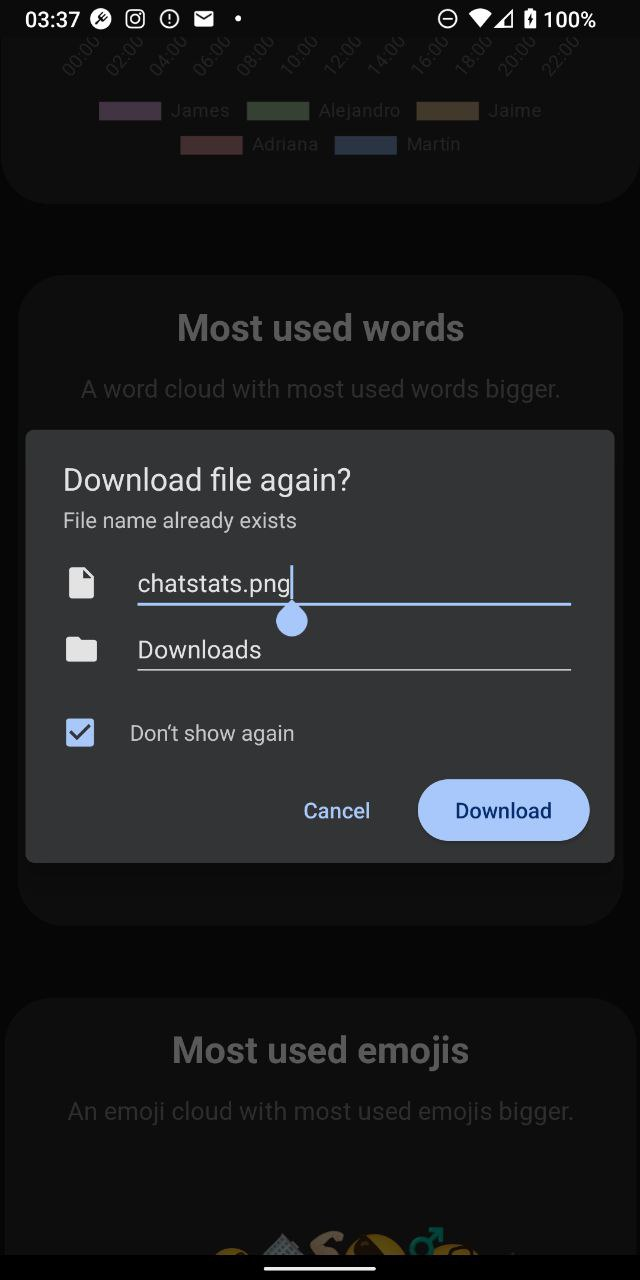
\includegraphics[width=5cm]{img/study_case/export_2.jpg} }}
	\caption{Exportar analíticas}
	\label{fig:chap5:export}
\end{figure}